% !TEX root=./adl.tex

% -----------------------------------------------------------------------
\begin{frame}{Limitations of Absolute Positional Encodings}

  Recall: sinusoidal or learned PE are \textbf{added} to token embeddings before attention.

  \vspace{0.5em}
  \textbf{Problems:}
  \begin{itemize}
    \item Attention scores depend on \emph{absolute} positions, not relative distance
    \item Sinusoidal PE: dot product $\text{PE}(m)^\top \text{PE}(n)$ depends on both $m$ and $n$, not just $m - n$
    \item Learned PE: cannot generalize beyond the maximum training length
    \item Adding PE to content embeddings mixes positional and semantic information
  \end{itemize}

  \vspace{0.5em}
  \begin{alertblock}{Desiderata}
    \begin{itemize}
      \item Attention score $\vq_m^\top \vk_n$ should depend on relative distance $m - n$
      \item Positional information should be \emph{injected into} Q and K, not added to content
      \item No learned parameters
    \end{itemize}
  \end{alertblock}

\end{frame}

% -----------------------------------------------------------------------
\begin{frame}{RoPE: Core Idea~\cite{su2024roformer}}

  \textbf{Key insight:} Encode position by \emph{rotating} query and key vectors.

  \vspace{0.3em}
  \begin{columns}[T]
    \begin{column}{0.52\textwidth}
      \begin{itemize}
        \item 2D subspace, position $m$, rotate by $m\theta$:
          \[
            R(m\theta) = \begin{pmatrix} \cos m\theta & -\sin m\theta \\ \sin m\theta & \cos m\theta \end{pmatrix}
          \]
          \vspace{-0.8em}
        \item Query and key at positions $m$, $n$:
          \[
            \tilde{\vq}_m = R(m\theta)\,\vq_m, \quad \tilde{\vk}_n = R(n\theta)\,\vk_n
          \]
          \vspace{-0.8em}
        \item Dot product:
          \vspace{-0.3em}
          \begin{align*}
            \tilde{\vq}_m^\top \tilde{\vk}_n &= \vq_m^\top R(m\theta)^\top R(n\theta)\,\vk_n \\
            &= \vq_m^\top R\bigl((n{-}m)\theta\bigr)\,\vk_n
          \end{align*}
          \vspace{-0.8em}
        \item Since $R(\alpha)^\top = R(-\alpha)$ (orthogonal):
          \vspace{-0.3em}
          \begin{align*}
            R(\alpha)^\top R(\beta) &= R(-\alpha)\,R(\beta) = R(\beta - \alpha)
          \end{align*}
      \end{itemize}
    \end{column}

    \begin{column}{0.45\textwidth}
      \begin{center}
      \begin{tikzpicture}[scale=0.92]
        % Axes
        \draw[-{Stealth[length=3pt]}, gray!50] (-2.3,0) -- (2.5,0);
        \draw[-{Stealth[length=3pt]}, gray!50] (0,-0.6) -- (0,2.5);

        % Unit circle (upper half)
        \draw[gray!25, dashed] (0,0) circle(2.0);

        % --- Angle definitions (chosen to avoid overlaps) ---
        \pgfmathsetmacro{\qang}{15}      % original q direction
        \pgfmathsetmacro{\mtheta}{55}    % q rotation = m*theta
        \pgfmathsetmacro{\qrot}{\qang + \mtheta}  % = 70

        \pgfmathsetmacro{\kang}{-40}     % original k direction
        \pgfmathsetmacro{\ntheta}{25}    % k rotation = n*theta
        \pgfmathsetmacro{\krot}{\kang + \ntheta}  % = -15

        % --- Original q (dashed) ---
        \draw[-{Stealth[length=4pt]}, blue!30, thick, dashed] (0,0) --
          ({2.0*cos(\qang)}, {2.0*sin(\qang)});
        \node[font=\tiny, blue!30, anchor=west] at
          ({2.05*cos(\qang)}, {2.0*sin(\qang)}) {$\vq_m$};

        % --- Rotated q (solid) ---
        \draw[-{Stealth[length=4pt]}, blue!70!black, thick] (0,0) --
          ({2.0*cos(\qrot)}, {2.0*sin(\qrot)});
        \node[font=\tiny, blue!70!black, anchor=south west] at
          ({2.0*cos(\qrot)+0.02}, {2.0*sin(\qrot)+0.02}) {$\tilde{\vq}_m$};

        % Arc for q rotation (inner, r=0.85)
        \draw[-{Stealth[length=2pt]}, blue!50, thick]
          ({0.85*cos(\qang)}, {0.85*sin(\qang)})
          arc[start angle=\qang, end angle=\qrot, radius=0.85];
        \node[font=\tiny, blue!50, anchor=south] at
          ({1.1*cos((\qang+\qrot)/2)}, {1.1*sin((\qang+\qrot)/2)}) {$m\theta$};

        % --- Original k (dashed) ---
        \draw[-{Stealth[length=4pt]}, orange!40, thick, dashed] (0,0) --
          ({2.0*cos(\kang)}, {2.0*sin(\kang)});
        \node[font=\tiny, orange!40, anchor=north] at
          ({2.0*cos(\kang)}, {2.0*sin(\kang)-0.1}) {$\vk_n$};

        % --- Rotated k (solid) ---
        \draw[-{Stealth[length=4pt]}, orange!70!black, thick] (0,0) --
          ({2.0*cos(\krot)}, {2.0*sin(\krot)});
        \node[font=\tiny, orange!70!black, anchor=north west] at
          ({2.0*cos(\krot)+0.05}, {2.0*sin(\krot)-0.08}) {$\tilde{\vk}_n$};

        % Arc for k rotation (innermost, r=0.6)
        \draw[-{Stealth[length=2pt]}, orange!50, thick]
          ({0.6*cos(\kang)}, {0.6*sin(\kang)})
          arc[start angle=\kang, end angle=\krot, radius=0.6];
        \node[font=\tiny, orange!50, anchor=west] at
          ({0.8*cos((\kang+\krot)/2)}, {0.8*sin((\kang+\krot)/2)}) {$n\theta$};

        % --- Angle between rotated vectors (outermost, r=1.5) ---
        \draw[{Stealth[length=2pt]}-{Stealth[length=2pt]}, red!60!black, thick]
          ({1.5*cos(\krot)}, {1.5*sin(\krot)})
          arc[start angle=\krot, end angle=\qrot, radius=1.5];
        \node[font=\scriptsize, red!60!black, anchor=south west] at
          ({1.7*cos((\qrot+\krot)/2)}, {1.7*sin((\qrot+\krot)/2)}) {$(n{-}m)\theta$};

      \end{tikzpicture}
      \end{center}
    \end{column}
  \end{columns}

  \vspace{0.3em}
  \begin{block}{Result}
    The attention score depends only on relative position $n - m$ and the content vectors.
  \end{block}

\end{frame}

% -----------------------------------------------------------------------
\begin{frame}{RoPE: Complex Number View}

  Equivalently, represent each dimension pair $(x_{2i}, x_{2i+1})$ as a complex number:
  \[
    z_i = x_{2i} + j\, x_{2i+1} \in \mathbb{C}
  \]

  RoPE at position $m$: multiply by a unit complex number
  \[
    \tilde{z}_i = z_i \cdot e^{j\, m \theta_i}
  \]

  \vspace{0.3em}
  The dot product between rotated queries and keys becomes:
  \[
    \operatorname{Re}\!\left(\tilde{z}_i^{(q)} \cdot \overline{\tilde{z}_i^{(k)}}\right) = \operatorname{Re}\!\left(z_i^{(q)} \cdot \overline{z_i^{(k)}} \cdot e^{j\,(m-n)\theta_i}\right)
  \]

  \vspace{0.3em}
  \begin{block}{Implementation in practice}
    \begin{itemize}
      \item Reshape Q, K into pairs: $(d/2)$ complex numbers
      \item Precompute $e^{j\, m \theta_i}$ for all positions $m$ and frequencies $i$
      \item Element-wise complex multiply (or equivalent real-valued formula)
    \end{itemize}
  \end{block}

\end{frame}

% -----------------------------------------------------------------------
\begin{frame}{RoPE: Full Rotation Matrix}

  For head dimension $d$, apply different rotation frequencies $\theta_i$ to each pair:
  \[
    \theta_i = \frac{1}{b^{2i/d}}, \quad i = 0, 1, \ldots, d/2 - 1
  \]
  where $b = 10{,}000$ is the base (same convention as sinusoidal PE).

  \vspace{0.3em}
  The full rotation matrix at position $m$ is block-diagonal:
  \[
    R_m = \begin{pmatrix}
      R(m\theta_0) & & \\
      & R(m\theta_1) & \\
      & & \ddots \\
      & & & R(m\theta_{d/2-1})
    \end{pmatrix}
  \]

  \vspace{0.3em}
  \begin{description}[labelwidth=\widthof{\bfseries High dimensions:~~}, leftmargin=!]
    \item[Low dimensions:] large $\theta_i$ $\Rightarrow$ fast rotation $\Rightarrow$ captures fine-grained local position
    \item[High dimensions:] small $\theta_i$ $\Rightarrow$ slow rotation $\Rightarrow$ captures long-range position
  \end{description}

  Analogous to the frequency spectrum in sinusoidal PE.

\end{frame}

% -----------------------------------------------------------------------
\begin{frame}{RoPE: Visualization}

  \begin{center}
  \begin{tikzpicture}[scale=0.85]

    % --- Left: 2D rotation diagram ---
    \begin{scope}[shift={(-3.2, 0)}]
      \draw[-{Stealth[length=3pt]}, gray!60] (-0.3,0) -- (2.5,0) node[right, font=\tiny, gray] {$x_{2i}$};
      \draw[-{Stealth[length=3pt]}, gray!60] (0,-0.3) -- (0,2.5) node[above, font=\tiny, gray] {$x_{2i+1}$};

      % Original vector
      \draw[-{Stealth[length=4pt]}, thick, blue!70!black] (0,0) -- (2.0, 0.73);
      \node[font=\scriptsize, blue!70!black, anchor=south west] at (2.0, 0.73) {$\vq_m$};

      % Rotated vector
      \draw[-{Stealth[length=4pt]}, thick, red!70!black] (0,0) -- (1.1, 1.82);
      \node[font=\scriptsize, red!70!black, anchor=south east] at (1.0, 1.9) {$\tilde{\vq}_m$};

      % Arc for angle
      \draw[-{Stealth[length=2.5pt]}, blue!50, thick] (1.36, 0.50) arc[start angle=20, end angle=59, radius=1.45];
      \node[font=\scriptsize, blue!50] at (1.55, 1.25) {$m\theta_i$};

      % Dashed circle
      \draw[gray!30, dashed] (0,0) circle(2.13);

      \node[font=\scriptsize, anchor=north] at (1.1, -0.4) {Rotation in pair $(2i, 2i{+}1)$};
    \end{scope}

    % --- Right: frequency spectrum ---
    \begin{scope}[shift={(1.8, -0.3)}]
      \node[font=\scriptsize, anchor=south] at (1.6, 2.5) {Rotation speed per dimension pair};

      \foreach \i/\speed/\col in {0/fast/red!70, 1/\phantom{x}/red!50, 2/\phantom{x}/orange!60, 3/\phantom{x}/yellow!70!orange, 4/\phantom{x}/green!50, 5/\phantom{x}/teal!50, 6/\phantom{x}/blue!40, 7/slow/blue!70} {
        \pgfmathsetmacro{\bw}{0.35}
        \pgfmathsetmacro{\bx}{\i * 0.43}
        \pgfmathsetmacro{\bh}{2.2 - \i * 0.25}
        \fill[\col] (\bx, 0) rectangle (\bx + \bw, \bh);
        \draw[gray!50, thin] (\bx, 0) rectangle (\bx + \bw, \bh);
        \node[font=\tiny, gray] at (\bx + \bw/2, -0.2) {$\i$};
      }

      \node[font=\tiny, red!70!black, anchor=west] at (3.7, 1.9) {local};
      \node[font=\tiny, blue!70!black, anchor=west] at (3.7, 0.5) {global};
      \draw[-{Stealth[length=2pt]}, gray!50, thin] (3.85, 1.7) -- (3.85, 0.7);

      \node[font=\tiny, gray] at (1.6, -0.4) {dimension pair index $i$};
    \end{scope}

  \end{tikzpicture}
  \end{center}

  \vspace{-0.5em}
  \begin{itemize}
    \item Each dimension pair is rotated independently at its own frequency
    \item Low-index pairs rotate fast (local patterns), high-index pairs rotate slowly (global patterns)
    \item Applied to Q and K \textbf{after} projection, \textbf{before} dot product
  \end{itemize}

\end{frame}

% -----------------------------------------------------------------------
\begin{frame}{RoPE: Properties}

  \begin{columns}[T]
    \begin{column}{0.52\textwidth}
      \begin{description}[labelwidth=\widthof{\bfseries No learned params:~~}, leftmargin=!]
        \item[Relative PE:] $\tilde{\vq}_m^\top \tilde{\vk}_n$ depends on $\vq_m$, $\vk_n$, and $m {-} n$ only
        \item[No learned params:] Fully determined by base $b$ and head dim $d$
        \item[Norm-preserving:] $\|R_m \vq\| = \|\vq\|$ (orthogonal)
        \item[Long-range decay:] As $|m{-}n|$ grows, rotating phases cancel $\Rightarrow$ inner product decays
        \item[Flexible:] Per-head, works with MHA, GQA, MQA
      \end{description}

      \vspace{0.3em}
      \begin{block}{Adoption}
        Used by LLaMA, Mistral, Qwen, Gemma, DeepSeek, and most modern open-weight LLMs.
      \end{block}
    \end{column}

    \begin{column}{0.46\textwidth}
      \textbf{Long-range decay} for unit vectors $\vq = \vk$:
      \vspace{-0.3em}
      \[
        \tilde{\vq}_m^\top \tilde{\vk}_n = \sum_{i=0}^{d/2-1} \cos\bigl((m{-}n)\,\theta_i\bigr)
      \]
      \vspace{-0.5em}

      \begin{center}
      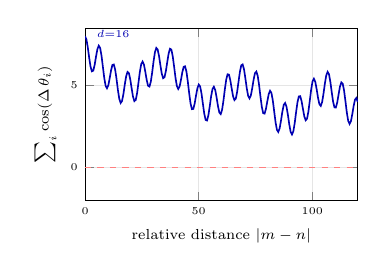
\begin{tikzpicture}[scale=0.75]
        \begin{axis}[
          width=6.2cm, height=4.5cm,
          xlabel={relative distance $|m - n|$},
          ylabel={$\sum_i \cos(\Delta\, \theta_i)$},
          xlabel style={font=\scriptsize},
          ylabel style={font=\scriptsize},
          tick label style={font=\tiny},
          xmin=0, xmax=120,
          ymin=-2, ymax=8.5,
          domain=0:120,
          samples=200,
          grid=major,
          grid style={gray!20},
          every axis plot/.append style={thick},
        ]
          % Sum of cos(delta * theta_i) for d=16 (8 pairs), base=10000
          % theta_i = 1/10000^(2i/16) for i=0..7
          \addplot[blue!70!black, thick] {
            cos(deg(x / 1.0))
            + cos(deg(x / 5.623))
            + cos(deg(x / 31.62))
            + cos(deg(x / 177.8))
            + cos(deg(x / 1000.0))
            + cos(deg(x / 5623.0))
            + cos(deg(x / 31623.0))
            + cos(deg(x / 100000.0))
          };

          % Reference line
          \draw[red!50, dashed, thin] (axis cs:0, 0) -- (axis cs:120, 0);

          % Annotations
          \node[font=\tiny, blue!70!black, anchor=south west] at (axis cs:2, 7.5) {$d{=}16$};
        \end{axis}
      \end{tikzpicture}
      \end{center}
      \vspace{-0.5em}
      {\scriptsize High-freq pairs oscillate and cancel; low-freq pairs decay slowly. Peak at $\Delta{=}0$ (all cosines $= 1$).}
    \end{column}
  \end{columns}

\end{frame}

% -----------------------------------------------------------------------
\begin{frame}{RoPE: Why Long-Range Decay?}

  Expand $\langle R_m \vq, R_n \vk\rangle$ pair by pair using $\cos(m\theta_i)\cos(n\theta_i) + \sin(m\theta_i)\sin(n\theta_i) = \cos(\Delta\theta_i)$, $\Delta = m-n$:
  \[
    \text{score}(m,n) = \sum_{i=0}^{d/2-1} a_i \cos(\Delta\,\theta_i) + b_i \sin(\Delta\,\theta_i)
  \]
  with, on each pair $(2i, 2i{+}1)$,
  \(
    a_i = q_{2i}k_{2i} + q_{2i+1}k_{2i+1}
  \)
  (unrotated dot product) and
  \(
    b_i = q_{2i+1}k_{2i} - q_{2i}k_{2i+1}
  \)
  (2D cross-product). Both are \textbf{content-only}; positions enter only through $\theta_i = \text{base}^{-2i/d}$.

  \vspace{0.3em}
  \begin{columns}[T]
    \begin{column}{0.55\textwidth}
      \textbf{$\Delta = 0$:} $\cos(0){=}1$, $\sin(0){=}0$ $\Rightarrow$ score $= \vq^\top \vk$ (full signal).

      \vspace{0.3em}
      \textbf{Growing $|\Delta|$:} pairs oscillate at different $\theta_i$; phases spread and \textbf{destructively interfere}:
      \begin{itemize}
        \item Small $|\Delta|$: high-freq pairs cancel; low-freq still coherent.
        \item Large $|\Delta|$: nearly all pairs incoherent; score near zero.
      \end{itemize}

      \vspace{0.3em}
      \textbf{Riemann-Lebesgue effect:} a sum of oscillators at spread-out frequencies vanishes as the phase shift grows.
    \end{column}
    \begin{column}{0.43\textwidth}
      \centering
      {\small\textbf{Phasor view} at large $|\Delta|$:}

      \begin{tikzpicture}[scale=0.45]
        % Unit circle
        \draw[gray!30] (0,0) circle(1.8);
        \draw[-{Stealth[length=2pt]}, gray!40] (-2.0,0) -- (2.0,0);
        \draw[-{Stealth[length=2pt]}, gray!40] (0,-2.0) -- (0,2.0);

        % Phasors at different angles (representing e^{j*Delta*theta_i} for various i)
        \foreach \ang/\col in {15/red!70, 72/orange!70, 145/yellow!70!black, 198/green!60!black, 253/teal!70, 290/blue!60, 340/violet!60, 50/red!40} {
          \draw[-{Stealth[length=2.5pt]}, \col, thick] (0,0) -- ({1.8*cos(\ang)},{1.8*sin(\ang)});
        }

        % Sum vector (small, near origin)
        \draw[-{Stealth[length=3pt]}, black, very thick] (0,0) -- (0.3, 0.15);
        \node[font=\tiny, anchor=west] at (0.35, 0.15) {$\sum$};

        \node[font=\tiny, gray, anchor=north] at (0, -2.0) {Phases spread $\Rightarrow$ sum $\approx 0$};
      \end{tikzpicture}

      {\small\textbf{At $\Delta = 0$} all phasors aligned:}

      \begin{tikzpicture}[scale=0.45]
        \draw[gray!30] (0,0) circle(1.8);
        \draw[-{Stealth[length=2pt]}, gray!40] (-2.0,0) -- (2.0,0);
        \draw[-{Stealth[length=2pt]}, gray!40] (0,-2.0) -- (0,2.0);

        % All phasors aligned to the right
        \foreach \i in {1,...,8} {
          \pgfmathsetmacro{\yoff}{(\i - 4.5) * 0.04}
          \draw[-{Stealth[length=2.5pt]}, blue!60, thick] (0,\yoff) -- (1.8,\yoff);
        }

        \draw[-{Stealth[length=3pt]}, black, very thick] (0,0) -- (1.8, 0);
        \node[font=\tiny, anchor=west] at (1.85, 0) {$\sum$};

        \node[font=\tiny, gray, anchor=north] at (0, -2.0) {All aligned $\Rightarrow$ max score};
      \end{tikzpicture}
    \end{column}
  \end{columns}
\end{frame}

% -----------------------------------------------------------------------
\begin{frame}{The Extrapolation Problem}

  RoPE is trained on sequences up to length $L_{\text{train}}$ (e.g.\ 4096 tokens).

  \vspace{0.3em}
  \textbf{At inference}, we want to handle $L_{\text{test}} \gg L_{\text{train}}$.

  \vspace{0.5em}
  \textbf{What goes wrong:}
  \begin{itemize}
    \item Positions $m > L_{\text{train}}$ produce rotation angles $m\theta_i$ never seen during training
    \item Attention logits become unpredictable for out-of-distribution positions
    \item Performance degrades sharply beyond training length
  \end{itemize}

  \vspace{0.5em}
  \textbf{Approaches:}
  \begin{description}[labelwidth=\widthof{\bfseries NTK-aware interpolation:~~}, leftmargin=!]
    \item[Position interpolation:] Scale positions: $m \to m \cdot \frac{L_{\text{train}}}{L_{\text{test}}}$~\cite{chen2023extending}. \\
      All angles stay in $[0, L_{\text{train}} \cdot \theta_i]$. Requires fine-tuning.
    \item[NTK-aware interpolation:] Scale the base $b$ instead of positions~\cite{bloc97_2023ntk}.
      Changes frequencies non-uniformly. Can work without fine-tuning.
    \item[YaRN:] Combines NTK-aware interpolation with attention scaling~\cite{peng2023yarn}.
  \end{description}

\end{frame}

% -----------------------------------------------------------------------
\begin{frame}{Position Interpolation vs.\ Extrapolation}

  Let $s = L_{\text{test}} / L_{\text{train}}$ be the scaling factor.

  \vspace{0.3em}
  \begin{columns}[T]
    \begin{column}{0.48\textwidth}
      \textbf{Extrapolation} (naive):
      \begin{itemize}
        \item Use original $\theta_i$ at all positions
        \item Positions $> L_{\text{train}}$: angles unseen during training
        \item High-frequency pairs: multiple full extra rotations
      \end{itemize}

      \vspace{0.3em}
      \begin{center}
      \begin{tikzpicture}[scale=0.65]
        % Axis
        \draw[-{Stealth[length=3pt]}, gray!60] (0,0) -- (5.5,0) node[right, font=\tiny] {position $m$};
        \draw[-{Stealth[length=3pt]}, gray!60] (0,0) -- (0,3.2) node[above, font=\tiny] {angle $m\theta_i$};

        % Training region
        \fill[green!15] (0,0) rectangle (2.5, 3.0);
        \node[font=\tiny, green!50!black] at (1.25, 2.7) {train};

        % Extrapolation region
        \fill[red!10] (2.5,0) rectangle (5.0, 3.0);
        \node[font=\tiny, red!50!black] at (3.75, 2.7) {unseen};

        % Line
        \draw[thick, blue!70] (0,0) -- (5.0, 3.0);
        \draw[dashed, gray] (2.5, 0) -- (2.5, 3.0);
      \end{tikzpicture}
      \end{center}
    \end{column}

    \begin{column}{0.48\textwidth}
      \textbf{Position Interpolation}:
      \begin{itemize}
        \item Scale: $m \to m/s$
        \item All angles map into training range
        \item Tokens are ``squeezed'' closer together
        \item Fine-tuning needed: model must adapt to denser positions
      \end{itemize}

      \vspace{0.3em}
      \begin{center}
      \begin{tikzpicture}[scale=0.65]
        % Axis
        \draw[-{Stealth[length=3pt]}, gray!60] (0,0) -- (5.5,0) node[right, font=\tiny] {position $m$};
        \draw[-{Stealth[length=3pt]}, gray!60] (0,0) -- (0,3.2) node[above, font=\tiny] {angle $m\theta_i / s$};

        % Training region
        \fill[green!15] (0,0) rectangle (5.0, 3.0);
        \node[font=\tiny, green!50!black] at (2.5, 2.7) {interpolated};

        % Line (shallower slope)
        \draw[thick, orange!70!black] (0,0) -- (5.0, 1.5);

        % Original line (dashed)
        \draw[dashed, blue!40] (0,0) -- (2.5, 1.5);
        \node[font=\tiny, blue!40, anchor=west] at (2.5, 1.7) {original};
      \end{tikzpicture}
      \end{center}
    \end{column}
  \end{columns}

\end{frame}

% -----------------------------------------------------------------------
\begin{frame}{NTK-aware Interpolation}

  \begin{description}[labelwidth=\widthof{\bfseries head dim $d$:~~}, leftmargin=!, font=\small]
    \item[scale $s$:] extension ratio $L_{\text{test}}/L_{\text{train}}$.
    \item[head dim $d$:] $d/2$ rotation pairs $i = 0,\ldots,\tfrac{d}{2}{-}1$ with frequencies $\theta_i = b^{-2i/d}$ and wavelengths $\lambda_i = 2\pi/\theta_i$.
  \end{description}

  \vspace{0.4em}
  \begin{columns}[T]
    \begin{column}{0.40\textwidth}
      \textbf{NTK-aware~\cite{bloc97_2023ntk}.} Scale the base, not positions:
      \[
        b' = b \cdot s^{\,d/(d-2)}.
      \]
      The exponent $\tfrac{d}{d-2}$ makes
      \begin{itemize}
        \item $\theta_0' = \theta_0$ (high freq kept),
        \item $\theta_{\tfrac{d}{2}-1}' = \theta_{\tfrac{d}{2}-1}/s$ (low freq fully interpolated).
      \end{itemize}

      \vspace{0.3em}
      Wavelengths shorter than $L_{\text{train}}$ stay; longer ones are stretched. Works without fine-tuning for $2$--$4\times$ extensions.
    \end{column}
    \begin{column}{0.58\textwidth}
      \centering
      \begin{tikzpicture}[scale=0.82,
          wbar/.style={line width=2.6pt, line cap=round},
          lbl/.style={font=\tiny},
        ]
        % Background regions: train, extension, beyond L_test
        \fill[green!10]  (0,   -0.1) rectangle (2.4, 4.7);
        \fill[orange!10] (2.4, -0.1) rectangle (4.8, 4.7);
        \fill[red!7]     (4.8, -0.1) rectangle (7.6, 4.7);

        % --- bars (drawn before dashed lines so the lines stay visible on top) ---
        % small i: tiny wavelength, NTK unchanged
        \draw[wbar, blue!70]         (0, 4.2)  -- (0.18, 4.2);
        \draw[wbar, orange!80!black] (0, 3.95) -- (0.18, 3.95);
        \node[lbl, anchor=west] at (0.4, 4.07) {small $i$ (high freq): unchanged};

        % medium-small i
        \draw[wbar, blue!70]         (0, 3.1)  -- (1.0, 3.1);
        \draw[wbar, orange!80!black] (0, 2.85) -- (1.3, 2.85);

        % medium i: near L_train, NTK crosses L_train
        \draw[wbar, blue!70]         (0, 2.0)  -- (2.0, 2.0);
        \draw[wbar, orange!80!black] (0, 1.75) -- (3.5, 1.75);

        % large i: long wavelength, heavy stretch
        \draw[wbar, blue!70]         (0, 0.85) -- (3.2, 0.85);
        \draw[wbar, orange!80!black] (0, 0.55) -- (6.6, 0.55);
        \node[lbl, anchor=west, orange!80!black] at (6.7, 0.55) {$\approx s\,\lambda_i$};
        \node[lbl, anchor=west] at (0.05, 0.25) {large $i$ (low freq): stretched};

        % Boundary markers (on top of bars)
        \draw[green!50!black, thick, densely dashed] (2.4, -0.1) -- (2.4, 4.7);
        \draw[red!50!black,   thick, densely dashed] (4.8, -0.1) -- (4.8, 4.7);
        \node[lbl, green!50!black, anchor=south] at (2.4, 4.7) {$L_{\text{train}}$};
        \node[lbl, red!50!black,   anchor=south] at (4.8, 4.7) {$L_{\text{test}}$};

        % Position axis (drawn last so it sits above fills)
        \draw[gray!60, -{Stealth[length=2.5pt]}] (-0.05, -0.1) -- (7.7, -0.1)
          node[right, lbl, gray] {position};

        % Side label
        \node[lbl, gray, rotate=90] at (-0.4, 2.5) {wavelength $\lambda_i$};

        % Legend
        \draw[wbar, blue!70]         (0.0, -0.75) -- (0.3, -0.75);
        \node[lbl, anchor=west] at (0.35, -0.75) {original $\lambda_i$};
        \draw[wbar, orange!80!black] (2.0, -0.75) -- (2.3, -0.75);
        \node[lbl, anchor=west] at (2.35, -0.75) {NTK $\lambda_i'$};
      \end{tikzpicture}
    \end{column}
  \end{columns}

\end{frame}

% -----------------------------------------------------------------------
\begin{frame}{YaRN: Yet another RoPE extensioN~\cite{peng2023yarn}}

  YaRN combines three ideas for robust context extension.

  \vspace{0.4em}
  \textbf{1. Frequency-dependent interpolation.}
  Let $r_i = L_{\text{train}}/\lambda_i$ be the number of full rotations of dim pair $i$ within the training context.

  \vspace{0.3em}
  \begin{columns}[T]
    \begin{column}{0.48\textwidth}
      \begin{description}[labelwidth=\widthof{\bfseries Interp.:~~}, leftmargin=!, font=\small]
        \item[Keep:] $r_i \ge \beta$ (high-freq, many cycles in $L_{\text{train}}$) -- $\theta_i$ unchanged.
        \item[Interp.:] $r_i \le \alpha$ (low-freq, $<\!1$ full cycle) -- $\theta_i \to \theta_i/s$.
        \item[Blend:] $\alpha < r_i < \beta$ -- linear ramp $\gamma(r_i)$.
      \end{description}

      \vspace{0.3em}
      \[
        \theta_i' = \bigl(1 - \gamma(r_i)\bigr)\,\frac{\theta_i}{s} + \gamma(r_i)\,\theta_i
      \]

      \vspace{0.2em}
      LLaMA defaults: $\alpha = 1$, $\beta = 32$.
    \end{column}
    \begin{column}{0.48\textwidth}
      \centering
      \begin{tikzpicture}[scale=0.9]
        % Background regions
        \fill[orange!10] (0,   0) rectangle (0.8, 1.9);
        \fill[gray!10]   (0.8, 0) rectangle (3.5, 1.9);
        \fill[blue!10]   (3.5, 0) rectangle (4.4, 1.9);

        % Region labels above plot
        \node[font=\tiny, orange!70!black] at (0.4, 2.10) {full interp.};
        \node[font=\tiny, gray!50!black]   at (2.15, 2.10) {blend};
        \node[font=\tiny, blue!50!black]   at (3.95, 2.10) {keep};

        % Axes
        \draw[gray!60, -{Stealth[length=3pt]}] (-0.05, 0) -- (4.7, 0)
          node[right, font=\tiny, gray] {$r_i$};
        \draw[gray!60, -{Stealth[length=3pt]}] (0, -0.05) -- (0, 2.5)
          node[above, font=\tiny, gray] {$\gamma(r_i)$};

        % Marks at α and β
        \draw[gray!50, densely dashed] (0.8, 0) -- (0.8, 1.7);
        \draw[gray!50, densely dashed] (3.5, 0) -- (3.5, 1.7);
        \node[font=\tiny, anchor=north] at (0.8, -0.02) {$\alpha$};
        \node[font=\tiny, anchor=north] at (3.5, -0.02) {$\beta$};

        % Horizontal reference at 1
        \draw[gray!40, densely dashed] (0, 1.7) -- (3.5, 1.7);
        \node[font=\tiny, gray, anchor=east] at (-0.05, 1.7) {$1$};
        \node[font=\tiny, gray, anchor=east] at (-0.05, 0) {$0$};

        % Ramp curve (drawn on top)
        \draw[blue!70!black, very thick]
          (0, 0) -- (0.8, 0) -- (3.5, 1.7) -- (4.4, 1.7);
      \end{tikzpicture}
    \end{column}
  \end{columns}

\end{frame}

% -----------------------------------------------------------------------
\begin{frame}{YaRN: Attention Scaling and Fine-Tuning}

  \textbf{2. Attention scaling} \\[0.3em]
  Interpolation compresses the angle differences, increasing attention logit magnitudes.

  \vspace{0.3em}
  YaRN compensates with a temperature factor:
  \[
    a_{m,n} = \frac{\tilde{\vq}_m^\top \tilde{\vk}_n}{\sqrt{d} \cdot t}
  \]
  where $t = \sqrt{0.1 \ln s + 1}$ (empirically determined).

  This restores the entropy of the attention distribution to match training behavior.

  \vspace{0.5em}
  \textbf{3. Fine-tuning} \\[0.3em]
  \begin{itemize}
    \item Only 400 steps of fine-tuning on long sequences needed
    \item $\sim$0.1\% of original training compute
    \item Achieves strong performance at $64\times$--$128\times$ extension
  \end{itemize}

  \vspace{0.5em}
  \begin{exampleblock}{Example: LLaMA 2}
    LLaMA 2 trained on 4K context. With YaRN: extends to 128K context
    while maintaining performance on short-context benchmarks.
  \end{exampleblock}

\end{frame}

% -----------------------------------------------------------------------
\begin{frame}{Context Extension: Summary}

  \begin{center}
  \begin{tabular}{l c c c}
    \toprule
    \textbf{Method} & \textbf{Fine-tuning} & \textbf{Max extension} & \textbf{Local resolution} \\
    \midrule
    Extrapolation (naive)    & None     & $\sim$1$\times$    & Preserved \\
    Position Interpolation   & Required & $\sim$8$\times$    & Reduced \\
    NTK-aware scaling        & Optional & $\sim$4$\times$    & Preserved \\
    \textbf{YaRN}            & Minimal  & $\sim$128$\times$  & Preserved \\
    \bottomrule
  \end{tabular}
  \end{center}

  \vspace{0.5em}
  \begin{block}{Takeaway}
    RoPE provides a clean, parameter-free relative positional encoding.
    Its rotation structure enables principled context length extension
    through frequency-aware interpolation (YaRN), making it the default
    choice in modern LLMs.
  \end{block}

\end{frame}
